\documentclass[conference]{IEEEtran}
\IEEEoverridecommandlockouts
\usepackage{amsmath,amssymb,booktabs,siunitx,cite,tikz,pgfplots,url}
\pgfplotsset{compat=1.18}
\sisetup{detect-all}
\title{When Do Flexible-Cable Dynamics Matter for Control?\\A Constraint-Aware Study of an Eight-Cable 6-DOF CDPR}
\author{\IEEEauthorblockN{M. J. Tachia}\IEEEauthorblockA{Affiliation to be completed for the conference submission\\Email to be added}}
\begin{document}
\maketitle
\begin{abstract}
Cable elasticity, distributed mass, and vibration can substantially affect cable-driven parallel robots (CDPRs), but increased model fidelity does not necessarily improve closed-loop control. This paper investigates when flexible-cable dynamics become significant for an eight-cable 6-DOF CDPR and whether explicit history-based compensation provides additional tracking benefit beyond a strong disturbance-observer controller under positive bounded cable tensions. A quasi-static elastic-catenary model is compared with a stateful reduced-order flexible-cable model to separate parameter-related and dynamic residuals. A validation-only excitation sweep shows that the dynamic-to-total force-residual magnitude ratio changes from approximately 0.09--0.16 at low excitation to above 0.90 in the high-frequency region of the tested benchmark. A gated recurrent unit estimator captures part of the fast dynamic residual, but its frequency-out-of-distribution force RMSE of 89.44 N is only modestly lower than the 94.13 N error obtained by assuming zero dynamic residual. In held-out constrained-control tests, a validation-tuned disturbance-observer QP controller outperforms the filtered DOB-plus-temporal-residual controller: the latter increases position RMSE by 8.99\%, 5.28\%, and 3.51\% in transition, high-frequency, and mixed-disturbance cases, respectively. High tension-constraint activity and nonzero wrench-allocation residuals further limit the conversion of improved dynamic information into tracking improvement. Flexible-dynamics significance, residual predictability, and available cable wrench should therefore be assessed together before explicit flexible-dynamics compensation is introduced.
\end{abstract}
\begin{IEEEkeywords}
cable-driven parallel robots, flexible cables, disturbance observer, constrained control, tension distribution, dynamic modeling
\end{IEEEkeywords}

\section{Introduction}
Cable-driven parallel robots (CDPRs) use lightweight cables to actuate a moving platform and can provide large workspaces with low moving inertia. Their control remains difficult because cables can only pull, actuation is redundant, the wrench that can be generated changes with pose, and long cables may exhibit sag, elasticity, distributed mass, and vibration \cite{Zarebidoki2022,TachiaReview2026}.

Many controllers simplify cables as straight, massless, or quasi-static elements because these assumptions make online computation practical. The validity of these simplifications depends on the task. Model-comparison studies show that accuracy and computational cost vary with the included cable effects \cite{Fabritius2023}. Experimental work on compliant CDPRs reports frequency-dependent vibration behavior \cite{Peng2023}, while flexible-cable control studies show that cable inertia and elastic modes become increasingly relevant as demanded motion bandwidth rises \cite{Bettega2023,Moussa2024,Saadaoui2025}. Recent vibration-control studies further demonstrate that elastic models can improve vibration suppression during demanding motion \cite{Zhao2025,Rousseau2026}.

A second line of work addresses model error without explicitly reconstructing all flexible dynamics. Disturbance observers, robust control, and model predictive control can reject lumped uncertainty while maintaining cable constraints \cite{Gao2025,Lu2024}. Learning-based methods have also been used to compensate cable sag and uncertain dynamics \cite{Tachia2025}. Temporal and gray-box identification has recently been used to improve high-frequency characterization while retaining physical structure \cite{Wang2026}. These developments raise a practical question: when flexible dynamics are physically significant, does explicit temporal compensation provide additional closed-loop benefit beyond a well-tuned disturbance observer?

The answer also depends on feasible cable forces. A desired platform wrench cannot always be generated by positive bounded tensions. Integrated nonlinear MPC, workspace-based MPC, and positive-constrained control therefore treat wrench feasibility as part of the control problem \cite{Santos2022,Song2022,Ameri2024}. Robust elastic-cable NMPC continues this direction by combining uncertainty rejection, elasticity, tension magnitude, and tension smoothness in a single constrained optimization \cite{Bellila2026}. Consequently, improved dynamic knowledge does not guarantee improved tracking if the corresponding corrective wrench cannot be produced by the cables.

This study addresses three questions: under what excitation conditions flexible-cable dynamics become a material component of model mismatch; whether history-based flexible-dynamics compensation provides additional tracking benefit beyond a validation-tuned disturbance observer; and how positive-tension and wrench-feasibility constraints affect the translation from improved dynamic information to improved tracking. The contribution is a matched computational comparison that treats these questions together rather than assuming that a larger model residual necessarily implies a larger control benefit.

\section{CDPR Model and Constrained Control Problem}
\subsection{Eight-Cable 6-DOF Dynamics}
Let $\mathbf a_i\in\mathbb R^3$ be the $i$th base anchor, $\mathbf b_i\in\mathbb R^3$ the corresponding platform attachment expressed in the platform frame, $\mathbf p$ the platform reference-point position, and $\mathbf R\in SO(3)$ its rotation matrix. The cable vector, length, and unit direction are
\begin{equation}
\mathbf l_i=\mathbf a_i-\mathbf p-\mathbf R\mathbf b_i,\quad
L_i=\|\mathbf l_i\|,\quad \mathbf u_i=\mathbf l_i/L_i .
\end{equation}
With $\mathbf r_i=\mathbf R\mathbf b_i$, the cable wrench is
\begin{equation}
\mathbf h_T=\mathbf W(\mathbf q)\mathbf T,\quad
\mathbf W=
\begin{bmatrix}
\mathbf u_1&\cdots&\mathbf u_8\\
\mathbf r_1\times\mathbf u_1&\cdots&\mathbf r_8\times\mathbf u_8
\end{bmatrix}.
\end{equation}
The rigid platform satisfies
\begin{align}
m\ddot{\mathbf p}&=\sum_{i=1}^{8}T_i\mathbf u_i+m\mathbf g,\\
\mathbf I_W\dot{\boldsymbol\omega}+\boldsymbol\omega\times(\mathbf I_W\boldsymbol\omega)
&=\sum_{i=1}^{8}\mathbf r_i\times T_i\mathbf u_i .
\end{align}

\begin{figure}[t]
\centering
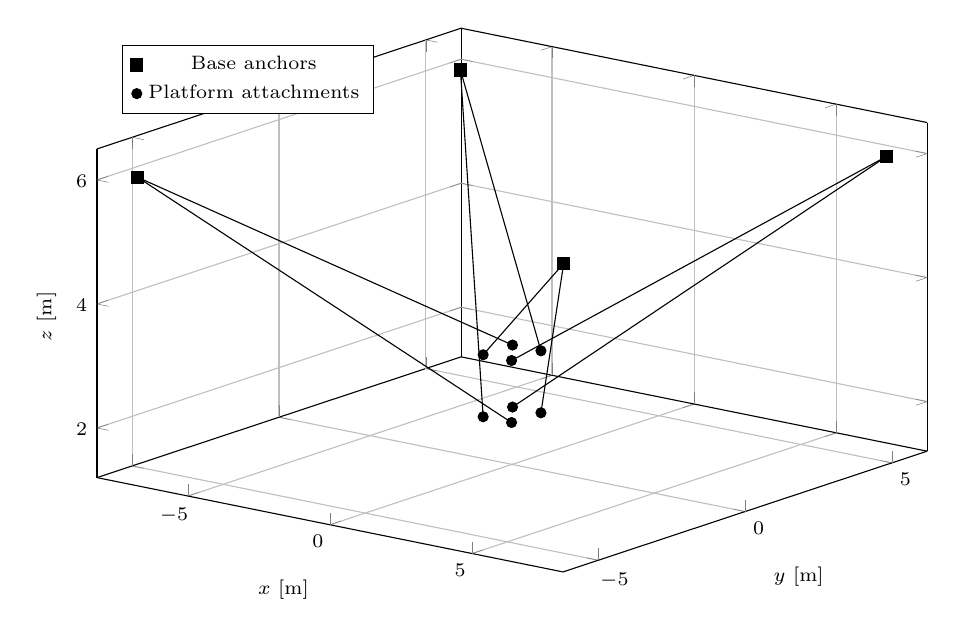
\begin{tikzpicture}
\begin{axis}[width=\columnwidth,height=0.70\columnwidth,view={38}{25},
xlabel={$x$ [m]},ylabel={$y$ [m]},zlabel={$z$ [m]},
xmin=-8.2,xmax=8.2,ymin=-6.2,ymax=6.2,zmin=1.2,zmax=6.5,
grid=major,legend style={font=\scriptsize,at={(0.03,0.97)},anchor=north west},
tick label style={font=\scriptsize},label style={font=\scriptsize}]
\addplot3[only marks,mark=square*,mark size=2.2pt] coordinates {(-7.5,-5.5,6) (-7.5,5.5,6) (7.5,5.5,6) (7.5,-5.5,6)};
\addlegendentry{Base anchors}
\addplot3[only marks,mark=*,mark size=1.8pt] coordinates {(0.5,-0.5,2) (-0.5,0.5,3) (-0.5,-0.5,2) (0.5,0.5,3) (-0.5,0.5,2) (0.5,-0.5,3) (0.5,0.5,2) (-0.5,-0.5,3)};
\addlegendentry{Platform attachments}
\addplot3[thin] coordinates {(0.5,-0.5,2) (-7.5,-5.5,6)};
\addplot3[thin] coordinates {(-0.5,0.5,3) (-7.5,-5.5,6)};
\addplot3[thin] coordinates {(-0.5,-0.5,2) (-7.5,5.5,6)};
\addplot3[thin] coordinates {(0.5,0.5,3) (-7.5,5.5,6)};
\addplot3[thin] coordinates {(-0.5,0.5,2) (7.5,5.5,6)};
\addplot3[thin] coordinates {(0.5,-0.5,3) (7.5,5.5,6)};
\addplot3[thin] coordinates {(0.5,0.5,2) (7.5,-5.5,6)};
\addplot3[thin] coordinates {(-0.5,-0.5,3) (7.5,-5.5,6)};
\end{axis}
\end{tikzpicture}
\caption{CoGiRo-inspired eight-cable 6-DOF benchmark geometry.}
\label{fig:geometry}
\end{figure}

\subsection{Quasi-Static and Stateful Cable Models}
The nominal model, denoted $L_1$, is an extensible quasi-static catenary accounting for cable weight, sag, and axial elasticity. The higher-fidelity reference, denoted $L_2$, retains the same mean catenary force and adds transverse assumed modes about the cable chord. Eight sine modes per cable were retained in the PAPER configuration. A generic modal coordinate satisfies
\begin{equation}
\ddot{\boldsymbol\eta}_{i,n}+2\zeta_{i,n}\omega_{i,n}\dot{\boldsymbol\eta}_{i,n}
+\omega_{i,n}^2\boldsymbol\eta_{i,n}=\mathbf f_{i,n}(t),
\end{equation}
with $\omega_{i,n}=n\pi L_i^{-1}\sqrt{T_i/\mu_i}$ in the reduced reference model. Modal displacement changes the endpoint tangent and includes the second-order small-slope geometric elongation used to obtain a dynamic tension increment. The first-mode sanity check at the nominal configuration was approximately \SI{3.74}{Hz}. Time-step and modal-truncation convergence tests were passed before data generation.

For analysis,
\begin{align}
\Delta\mathbf h_{\rm par}&=\mathbf h_{L_1}^{\rm true}-\mathbf h_{L_1}^{\rm nom},\\
\Delta\mathbf h_{\rm dyn}&=\mathbf h_{L_2}^{\rm true}-\mathbf h_{L_1}^{\rm true},\\
\Delta\mathbf h_{\rm tot}&=\Delta\mathbf h_{\rm par}+\Delta\mathbf h_{\rm dyn}.
\end{align}
True cable parameters and modal states are used only by the reference plant and for analysis.

\subsection{Positive-Tension Allocation}
The required wrench is converted into tensions through a normalized quadratic program,
\begin{equation}
\mathbf T^\star=\arg\min_{\mathbf T}
\|\mathbf S(\mathbf W\mathbf T-\mathbf h_{\rm cmd})\|_{\mathbf Q}^{2}
+\lambda_{\Delta T}\|\mathbf T-\mathbf T_{k-1}\|_2^2 ,
\end{equation}
subject to $T_{\min}\le T_i\le T_{\max}$. The scaling matrix $\mathbf S$ normalizes force and moment terms. If the requested wrench cannot be reproduced under the tension bounds, a nonzero normalized wrench residual remains. This quantity measures allocation infeasibility, not physical cable slack.

\section{Computational Methodology}
The geometry and unloaded platform mass are based on published CoGiRo data \cite{ElGhazaly2014}; cable diameter, linear density, low-force effective axial rigidity, and winch capability use a later CoGiRo cable characterization \cite{Izard2017}. The system is therefore a CoGiRo-inspired numerical benchmark rather than a digital twin of one hardware revision.

\begin{table}[t]
\caption{Main Benchmark Parameters}
\centering\footnotesize
\begin{tabular}{lll}
\toprule
Quantity & Value & Status\\
\midrule
Frame size & $15\times11\times6$ m & published\\
Platform mass & 79 kg & published\\
Cable diameter & 4 mm & published\\
Linear density & 0.0685 kg/m & published\\
Effective $EA$ & 339 kN & published\\
Minimum tension & 150 N & study setting\\
Ordinary $T_{\max}$ & 1500 N & study setting\\
Boundary $T_{\max}$ & 900 N & stress setting\\
Winch capability & 4150 N & published\\
Plant / control rate & 100 / 50 Hz & study setting\\
\bottomrule
\end{tabular}
\end{table}

A validation-only excitation sweep from 0.5 to \SI{4.5}{Hz} was used to characterize the relative importance of stateful dynamics,
\begin{equation}
\rho_{\rm dyn}=
\frac{\mathrm{RMS}\left(\|\Delta\mathbf F_{\rm dyn}\|_2\right)}
{\mathrm{RMS}\left(\|\Delta\mathbf F_{\rm tot}\|_2\right)+\varepsilon}.
\end{equation}
Because parameter and dynamic residual vectors can partially cancel, $\rho_{\rm dyn}$ is treated as a dynamic-to-total residual magnitude ratio, not an energy fraction.

\begin{figure}[t]
\centering
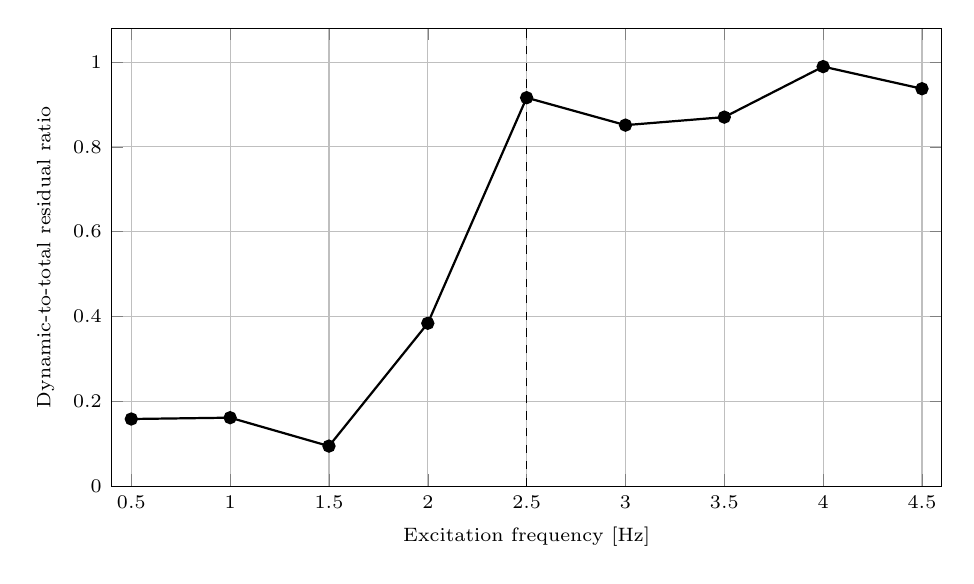
\begin{tikzpicture}
\begin{axis}[width=\columnwidth,height=0.61\columnwidth,
xlabel={Excitation frequency [Hz]},ylabel={Dynamic-to-total residual ratio},
xmin=0.4,xmax=4.6,ymin=0,ymax=1.08,
xtick={0.5,1,1.5,2,2.5,3,3.5,4,4.5},grid=both,
tick label style={font=\scriptsize},label style={font=\scriptsize}]
\addplot[mark=*,thick] coordinates {(0.5,0.15823) (1.0,0.16137) (1.5,0.09433) (2.0,0.38409) (2.5,0.91611) (3.0,0.85140) (3.5,0.87032) (4.0,0.98946) (4.5,0.93724)};
\addplot[dashed] coordinates {(2.5,0) (2.5,1.08)};
\end{axis}
\end{tikzpicture}
\caption{Dynamic-to-total force-residual magnitude ratio over the validation excitation sweep.}
\label{fig:residualmap}
\end{figure}

Five controller configurations use the same feedback structure and tension allocator: catenary-QP, DOB-QP, GRU residual-QP, DOB+GRU-QP, and filtered DOB+GRU-QP. The recurrent estimator processes a 0.5 s history at 50 Hz and uses only controller-available platform and cable features. Hidden cable parameters and modal states are excluded. Five independently trained model seeds were rotated through held-out trials.

The DOB cutoff and residual crossover were frozen before final testing. Validation selected a \SI{1}{Hz} DOB cutoff, a \SI{2.5}{Hz} residual crossover, and DOB-QP as the strongest fixed comparator. Six held-out cases were tested: nominal motion, slow model uncertainty, a 0.6--\SI{4.2}{Hz} chirp, high-frequency excitation around 3.4--\SI{4.1}{Hz}, combined dynamic excitation and disturbance, and a boundary case designed to activate tension limits. Each principal condition used 20 paired trials. Bootstrap confidence intervals used 4000 resamples, and paired Wilcoxon tests were adjusted using the Holm procedure.

\section{Results}
\subsection{When Flexible Dynamics Become Significant}
At 0.5, 1.0, and \SI{1.5}{Hz}, the median ratios in Fig.~\ref{fig:residualmap} were 0.158, 0.161, and 0.094. The value increased to 0.384 at \SI{2}{Hz} and 0.916 at \SI{2.5}{Hz}. Ratios remained above 0.85 from 3 to \SI{4.5}{Hz}, with a maximum of 0.989 at \SI{4}{Hz}. The dynamic force-residual RMS reached \SI{41.64}{N} at \SI{4.5}{Hz}.

The residual decomposition gives the same physical picture. In the moderate transient set, the parameter-related force residual was \SI{19.98}{N} RMS while the dynamic contribution was only \SI{1.07}{N}. In the frequency-out-of-distribution set, the parameter component was \SI{21.41}{N}, whereas the dynamic component increased to \SI{90.49}{N}. Flexible-cable dynamics are therefore not uniformly important. The observed transition near \SI{2.5}{Hz} is specific to the present benchmark.

\subsection{Temporal Prediction of the Dynamic Residual}
The recurrent model had lower validation loss than the memoryless estimator, confirming that history contains useful information. The harder control-relevant comparison is against the zero-dynamic-residual assumption.

\begin{table}[t]
\caption{Dynamic Residual and Force Prediction RMSE}
\centering\footnotesize
\begin{tabular}{lrrrr}
\toprule
Split & Param. & Dynamic & Zero & GRU\\
 & \multicolumn{2}{c}{residual RMS [N]} & \multicolumn{2}{c}{RMSE [N]}\\
\midrule
Transient & 19.98 & 1.07 & \textbf{1.08} & 7.04\\
IID & 15.66 & 26.80 & \textbf{27.89} & 31.29\\
Freq. OOD & 21.41 & \textbf{90.49} & 94.13 & \textbf{89.44}\\
Param. OOD & \textbf{105.25} & 26.78 & \textbf{27.85} & 29.01\\
\bottomrule
\end{tabular}
\end{table}

The GRU provides a modest improvement only in the frequency-OOD condition, where the dynamic component dominates. Its improvement relative to zero residual is about 5\%. In the moderate transient, zero compensation gives \SI{1.08}{N} RMSE, while the GRU increases error to \SI{7.04}{N}. Physical significance and causal prediction quality are therefore distinct requirements.

\subsection{Closed-Loop Comparison Against DOB-QP}
DOB-QP was selected as the strongest fixed controller before held-out testing.

\begin{table*}[t]
\caption{Held-Out Position Tracking Performance}
\centering\footnotesize
\begin{tabular}{lrrrrrr}
\toprule
Scenario & Catenary-QP & DOB-QP & GRU-QP & DOB+GRU & Filtered DOB+GRU & Change vs. DOB\\
 & \multicolumn{5}{c}{Primary position RMSE [m]} & [\%]\\
\midrule
Nominal & 0.05746 & \textbf{0.05329} & 0.05712 & 0.05420 & 0.05330 & $-0.07$\\
Slow uncertainty & 0.11172 & 0.05473 & 0.11113 & 0.06499 & \textbf{0.05456} & $+0.31$\\
Transition chirp & 0.09390 & \textbf{0.07915} & 0.11196 & 0.09992 & 0.08533 & $-8.99$\\
High-frequency & 0.21445 & \textbf{0.19965} & 0.21279 & 0.20359 & 0.20884 & $-5.28$\\
Mixed disturbance & 0.17972 & \textbf{0.14625} & 0.17250 & 0.14789 & 0.15138 & $-3.51$\\
\bottomrule
\end{tabular}
\end{table*}

\begin{figure}[t]
\centering
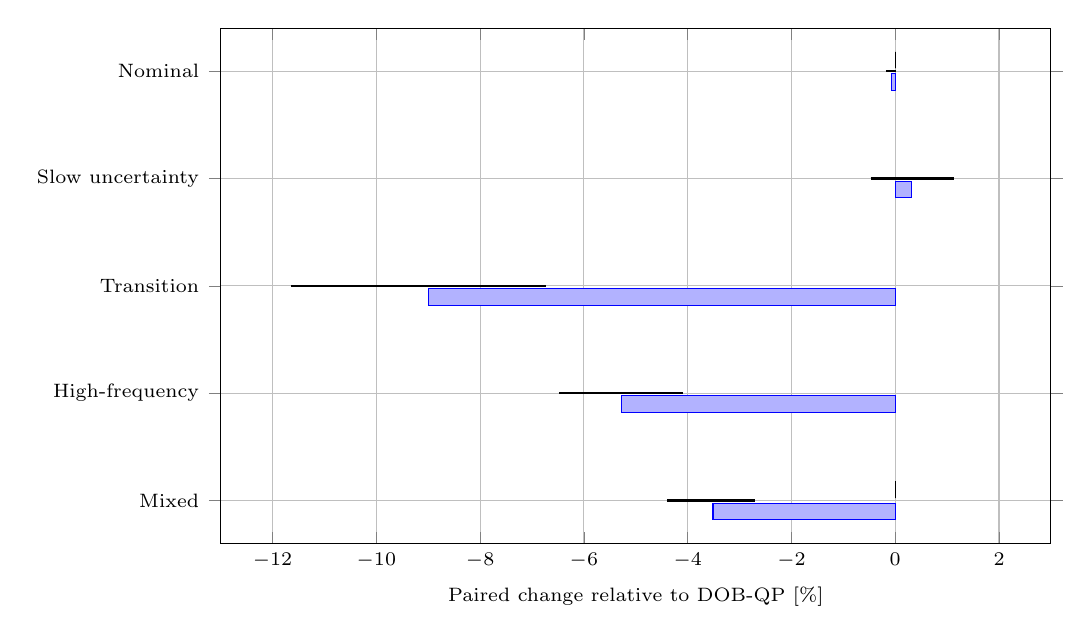
\begin{tikzpicture}
\begin{axis}[width=\columnwidth,height=0.67\columnwidth,xbar,
xmin=-13,xmax=3,xlabel={Paired change relative to DOB-QP [\%]},
symbolic y coords={Mixed,High-frequency,Transition,Slow uncertainty,Nominal},ytick=data,
grid=both,tick label style={font=\scriptsize},label style={font=\scriptsize},bar width=6pt]
\addplot coordinates {(-3.513,Mixed) (-5.278,High-frequency) (-8.993,Transition) (0.309,Slow uncertainty) (-0.075,Nominal)};
\draw[thick] (axis cs:-4.397,Mixed) -- (axis cs:-2.698,Mixed);
\draw[thick] (axis cs:-6.481,High-frequency) -- (axis cs:-4.090,High-frequency);
\draw[thick] (axis cs:-11.649,Transition) -- (axis cs:-6.734,Transition);
\draw[thick] (axis cs:-0.476,Slow uncertainty) -- (axis cs:1.136,Slow uncertainty);
\draw[thick] (axis cs:-0.179,Nominal) -- (axis cs:0.019,Nominal);
\addplot[dashed] coordinates {(0,Mixed) (0,Nominal)};
\end{axis}
\end{tikzpicture}
\caption{Paired position-RMSE change of filtered DOB+GRU compensation relative to DOB-QP; horizontal lines show 95\% bootstrap confidence intervals.}
\label{fig:control}
\end{figure}

The filtered controller is statistically indistinguishable from DOB-QP in nominal and slow-uncertainty cases. It increases position RMSE by 8.99\% in the transition chirp, 5.28\% in the high-frequency case, and 3.51\% under mixed disturbance. Their 95\% confidence intervals are entirely below zero, and one-sided paired tests did not support superiority after Holm correction.

The comparator changes the interpretation. Relative to catenary-QP, the filtered controller improves transition and mixed-disturbance tracking by 13.05\% and 16.10\%, respectively. Those gains disappear against the stronger DOB-QP comparator. Thus, a large flexible-dynamics residual is insufficient evidence that explicit temporal compensation provides incremental benefit beyond an already effective observer.

\subsection{Tension Feasibility and Control Performance}
All 120 held-out trials of the filtered controller completed, with zero commanded tension-bound violations. The lowest actual tension was \SI{152.89}{N}, and the largest was \SI{932.32}{N}, below the published \SI{4150}{N} winch capability. Constraint activity increased with dynamic demand: 0.001 in nominal operation, 0.164 in transition, 0.286 in the high-frequency case, 0.259 under mixed disturbance, and 0.446 in the boundary test.

The p95 normalized QP wrench residual increased from 0.0069 in nominal operation to 0.363, 0.699, and 0.384 in transition, high-frequency, and mixed cases. The learned fast correction also remained small relative to the true dynamic-force magnitude, with mean magnitude ratios of approximately 0.214, 0.162, and 0.197.

\begin{figure}[t]
\centering
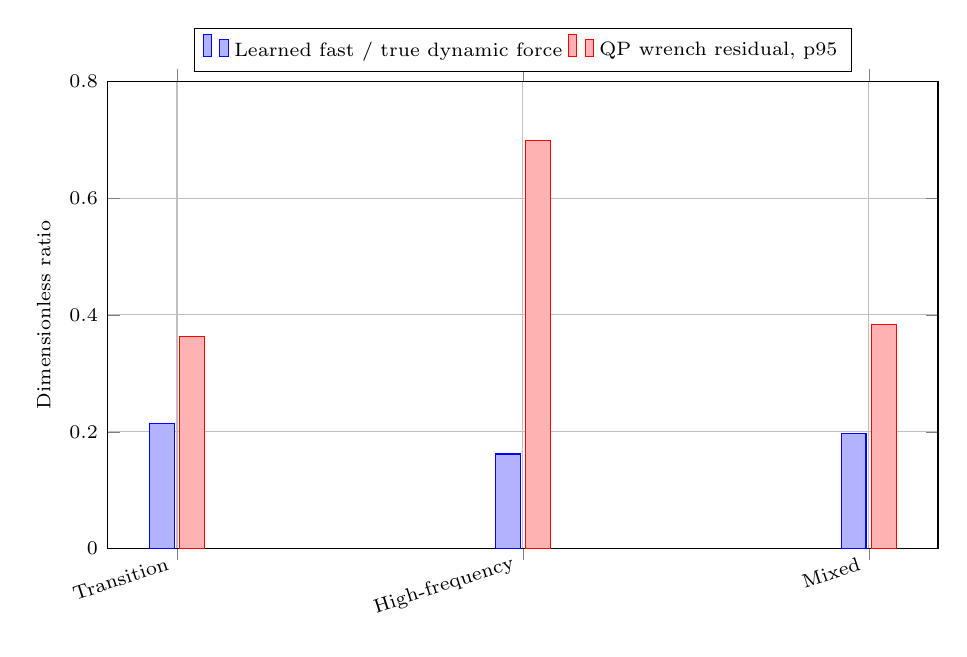
\begin{tikzpicture}
\begin{axis}[width=\columnwidth,height=0.62\columnwidth,ybar,bar width=9pt,
ymin=0,ymax=0.8,ylabel={Dimensionless ratio},
symbolic x coords={Transition,High-frequency,Mixed},xtick=data,
xticklabel style={font=\scriptsize,rotate=18,anchor=east},
tick label style={font=\scriptsize},label style={font=\scriptsize},
legend style={font=\scriptsize,at={(0.5,1.02)},anchor=south,legend columns=2},grid=major]
\addplot coordinates {(Transition,0.214) (High-frequency,0.162) (Mixed,0.197)};
\addlegendentry{Learned fast / true dynamic force}
\addplot coordinates {(Transition,0.363) (High-frequency,0.699) (Mixed,0.384)};
\addlegendentry{QP wrench residual, p95}
\end{axis}
\end{tikzpicture}
\caption{Scale of learned fast correction and normalized QP wrench residual in the three dynamic test cases.}
\label{fig:feasibility}
\end{figure}

Tension-rate RMS increased from 1046 to \SI{1112}{N/s} in transition, from 2072 to \SI{2215}{N/s} in the high-frequency case, and from 1696 to \SI{1857}{N/s} under mixed disturbance when temporal correction was added to DOB. The filtered controller reduced 2.5--\SI{5.5}{Hz} position-error power relative to DOB by about 10.3\%, 7.0\%, and 2.4\%, respectively, but these reductions did not coincide with lower total trajectory RMSE. The largest ordinary-condition p95 compensation-and-allocation time was \SI{18.50}{ms}; the boundary case reached \SI{19.24}{ms}, consistent with the selected 50 Hz update in the tested environment.

\section{Discussion}
The first result is that flexible-cable dynamics are strongly operating-condition dependent. This agrees with studies showing that cable inertia, elasticity, and vibration become increasingly relevant as excitation approaches flexible modes \cite{Peng2023,Saadaoui2025,Rousseau2026}. The present residual decomposition adds a direct comparison between quasi-static parameter mismatch and stateful dynamics on the same eight-cable benchmark.

The second result is the distinction between model importance and control benefit. Temporal information improves frequency-OOD residual prediction, but the improvement over a zero-dynamic-residual baseline is modest and does not generalize to all splits. In closed loop, the validation-tuned DOB-QP controller remains better in every primary dynamic case. This is consistent with the wider literature: explicit elastic models can improve vibration suppression \cite{Rousseau2026,Bellila2026}, while observer-based control can reject substantial lumped uncertainty under tension constraints \cite{Gao2025}. A large fast residual alone therefore does not justify an additional learned correction.

The third result is that available cable wrench limits how model information can be used. Difficult dynamic tests contain substantial active-bound fractions and nonzero QP wrench residuals, while the learned correction increases tension-rate demand. Before introducing explicit flexible-dynamics compensation, three conditions should therefore be checked: the omitted dynamics must be materially important, they must be predictable from available measurements, and the corresponding corrective wrench must be realizable within positive bounded tensions.

Three limitations are important. First, the conclusions come from a reduced-order computational benchmark rather than a physical eight-cable robot, so absolute transition frequencies and residual amplitudes are system dependent. Second, the final held-out study evaluates one principal temporal architecture, so the result does not represent every possible learning method. Third, feasibility results depend partly on the selected tension allocator and software bounds. The next useful step is experimental validation of the same control-headroom test on a physical CDPR.

\section{Conclusion}
This study investigated when flexible-cable dynamics become relevant to constrained control of an eight-cable 6-DOF CDPR and whether explicit history-based compensation provides additional benefit beyond disturbance observation. The dynamic-to-total force-residual magnitude ratio is small under low excitation and exceeds 0.9 in the high-frequency region of the tested benchmark, confirming that required cable-model fidelity depends on operating conditions.

That physical importance does not translate automatically into closed-loop benefit. Although the recurrent estimator captures part of the high-frequency residual, DOB-QP remains the strongest controller in the held-out transition, high-frequency, and mixed-disturbance cases. The filtered DOB+GRU controller increases position RMSE by 8.99\%, 5.28\%, and 3.51\% relative to DOB-QP.

High dynamic excitation also increases active tension constraints, wrench-allocation residuals, and tension-rate demand, while the learned fast correction remains an imperfect estimate of the true dynamic contribution. Explicit flexible-dynamics compensation should therefore be justified not by model-mismatch magnitude alone, but by the combination of dynamic significance, prediction quality, and attainable cable wrench.

\begin{thebibliography}{20}
\bibitem{Zarebidoki2022} M. Zarebidoki, J. S. Dhupia, and W. Xu, "A review of cable-driven parallel robots: Typical configurations, analysis techniques, and control methods," \emph{IEEE Robot. Autom. Mag.}, vol. 29, pp. 89--106, 2022, doi: 10.1109/MRA.2021.3138387.
\bibitem{TachiaReview2026} M. J. Tachia and A. V. Maloletov, "Applications of dynamic models for cable-driven parallel robots: A comprehensive review," \emph{Russian J. Nonlinear Dyn.}, vol. 22, no. 1, pp. 139--200, 2026, doi: 10.20537/nd251101.
\bibitem{Fabritius2023} M. Fabritius, P. Miermeister, W. Kraus, and A. Pott, "A framework for analyzing the accuracy, complexity, and long-term performance of cable-driven parallel robot models," \emph{Mech. Mach. Theory}, vol. 185, Art. no. 105331, 2023, doi: 10.1016/j.mechmachtheory.2023.105331.
\bibitem{Peng2023} M.-J. Peng, L.-H. Xiao, Q.-L. Chen, G.-W. Wei, Q. Lin, and J. Zhuo, "Dynamic modeling and characterization of compliant cable-driven parallel robots containing flexible cables," \emph{Robotica}, vol. 41, no. 10, pp. 3160--3174, 2023, doi: 10.1017/S0263574723000930.
\bibitem{Bettega2023} J. Bettega, G. Piva, D. Richiedei, and A. Trevisani, "Model predictive control for path tracking in cable driven parallel robots with flexible cables: Collocated vs. noncollocated control," \emph{Multibody Syst. Dyn.}, vol. 58, pp. 47--81, 2023, doi: 10.1007/s11044-023-09881-0.
\bibitem{Moussa2024} K. Moussa, A. Vié, M. Thieffry, F. Claveau, and P. Chevrel, "Model predictive control of cable-driven parallel robot with cable sagging: An assumed mode approach," in \emph{Proc. 28th Int. Conf. System Theory, Control and Computing}, 2024, pp. 533--538, doi: 10.1109/ICSTCC62912.2024.10744726.
\bibitem{Saadaoui2025} R. Saadaoui, O. Piccin, G. I. Bara, and É. Laroche, "Modeling and control of a 3-DOF planar cable-driven parallel robot with flexible cables," \emph{J. Dyn. Syst., Meas., Control}, vol. 147, no. 5, Art. no. 051009, 2025, doi: 10.1115/1.4068250.
\bibitem{Zhao2025} X. Zhao, J. Du, and K. Zhao, "Vibration suppression of redundantly controlled cable-driven parallel robots," \emph{Robot. Auton. Syst.}, vol. 183, Art. no. 104838, 2025, doi: 10.1016/j.robot.2024.104838.
\bibitem{Rousseau2026} S. Rousseau, N. Pedemonte, F. Chaumette, and S. Caro, "Model-predictive vibration reduction of a suspended cable-driven parallel robot," \emph{IEEE Robot. Autom. Lett.}, vol. 11, pp. 6744--6751, 2026, doi: 10.1109/LRA.2026.3681158.
\bibitem{Wang2026} R. Wang, Y.-M. Li, and Y. Zeng, "A gray-box identification method for cable-driven parallel robots via wavelet-enhanced neural networks," \emph{Robotica}, vol. 44, no. 2, pp. 612--629, 2026, doi: 10.1017/S0263574726103221.
\bibitem{Tachia2025} M. J. Tachia and A. V. Maloletov, "Reinforcement learning-based control for cable sag compensation in cable-driven parallel robots using soft actor-critic algorithm," in \emph{Proc. 2025 VI Int. Conf. Control in Technical Systems}, 2025, pp. 171--176, doi: 10.1109/CTS67336.2025.11196696.
\bibitem{Gao2025} X.-Y. Gao, W.-W. Shang, and B. Zhang, "Disturbance observer-based model predictive control for cable-driven parallel robots," \emph{IEEE Trans. Robot.}, vol. 41, pp. 6307--6326, 2025, doi: 10.1109/TRO.2025.3626664.
\bibitem{Lu2024} Y.-Q. Lu, W. Yao, C. Wu, X.-L. Li, and G.-H. Sun, "Disturbance observer-based control for cable-driven parallel robots with external disturbance using deep reinforcement learning," \emph{Asian J. Control}, vol. 26, pp. 2523--2538, 2024, doi: 10.1002/asjc.3353.
\bibitem{Santos2022} J. C. Santos, M. Gouttefarde, and A. Chemori, "A nonlinear model predictive control for the position tracking of cable-driven parallel robots," \emph{IEEE Trans. Robot.}, vol. 38, no. 4, pp. 2597--2616, 2022, doi: 10.1109/TRO.2022.3152705.
\bibitem{Song2022} C. Song and D. Lau, "Workspace-based model predictive control for cable-driven robots," \emph{IEEE Trans. Robot.}, vol. 38, pp. 2577--2596, 2022, doi: 10.1109/TRO.2021.3139585.
\bibitem{Ameri2024} A. Ameri, S. M. Fazeli, A. Molaei, M. A. Khosravi, and M. Hassani, "Noniterative positive constrained control of cable-driven parallel robots," \emph{IEEE Trans. Ind. Informat.}, vol. 20, pp. 2007--2016, 2024, doi: 10.1109/TII.2023.3285038.
\bibitem{Bellila2026} A. N. Bellila, M. Gouttefarde, H. Chanal, O. Company, and C. Bouzgarrou, "Nonlinear MPC with embedded super-twisting sliding modes for robust control of elastic cable-driven parallel robots," \emph{Mech. Mach. Theory}, vol. 229, Art. no. 106569, 2026, doi: 10.1016/j.mechmachtheory.2026.106569.
\bibitem{ElGhazaly2014} G. El-Ghazaly, M. Gouttefarde, and V. Creuze, "Adaptive terminal sliding mode control of a redundantly-actuated cable-driven parallel manipulator: CoGiRo," in \emph{Cable-Driven Parallel Robots}, 2014, pp. 179--200, doi: 10.1007/978-3-319-09489-2\_13.
\bibitem{Izard2017} J.-B. Izard, A. Dubor, P.-E. Hervé, E. Cabay, D. Culla, M. Rodriguez, and M. Barrado, "On the improvements of a cable-driven parallel robot for achieving additive manufacturing for construction," in \emph{Cable-Driven Parallel Robots}, vol. 53, pp. 353--363, 2017, doi: 10.1007/978-3-319-61431-1\_30.
\end{thebibliography}
\end{document}
